% Straight up stealing preamble from Eli Holmes 
%%%%%%%%%%%%%%%%%%%%%%%%%%%%%%%%%%%%%%START PREAMBLE THAT IS THE SAME FOR ALL EXAMPLES
\documentclass{article}

%Required: You must have these
\usepackage{Sweave}
\usepackage{graphicx}
\usepackage{tabularx}
\usepackage{hyperref}
\usepackage{natbib}
\usepackage{pdflscape}
\usepackage{array}
\usepackage{gensymb}

%\usepackage[backend=bibtex]{biblatex}
%Strongly recommended
 %put your figures in one place
 
%you'll want these for pretty captioning
\usepackage[small]{caption}

\setkeys{Gin}{width=0.8\textwidth} %make the figs 50 perc textwidth
\setlength{\captionmargin}{30pt}
\setlength{\abovecaptionskip}{0pt}
\setlength{\belowcaptionskip}{10pt}
% manual for caption http://www.dd.chalmers.se/latex/Docs/PDF/caption.pdf

%Optional: I like to muck with my margins and spacing in ways that LaTeX frowns on
%Here's how to do that
 \topmargin -2cm     
 \oddsidemargin -0.04cm   
 \evensidemargin -0.04cm  % same as oddsidemargin but for left-hand pages
 \textwidth 16.59cm
 \textheight 22.94cm 
 %\pagestyle{empty}       % Uncomment if don't want page numbers
 \parskip 7.2pt           % sets spacing between paragraphs
 %\renewcommand{\baselinestretch}{1.5} 	% Uncomment for 1.5 spacing between lines
\parindent 0pt% sets leading space for paragraphs
\usepackage{setspace}
%\doublespacing

%Optional: I like fancy headers
\usepackage{fancyhdr}
\pagestyle{fancy}
\fancyhead[LO]{Phenological sequences}
\fancyhead[RO]{2017}

%%%%%%%%%%%%%%%%%%%%%%%%%%%%%%%%%%%%%%END PREAMBLE THAT IS THE SAME FOR ALL EXAMPLES

%Start of the document
\begin{document}

% \SweaveOpts{concordance=TRUE}
\bibliographystyle{/Users/aileneettinger/citations/Bibtex/styles/amnat.bst}
\title{Supplemental materials for \\ Phenological sequences: How early-season events define those that follow} 
\author{A.K. Ettinger, S. Gee, and E.M. Wolkovich}
%\date{\today}
\maketitle  %put the fancy title on
%\tableofcontents      %add a table of contents
%\clearpage
%%%%%%%%%%%%%%%%%%%%%%%%%%%%%%%%%%%%%%%%%%%%%%%%%%%
\renewcommand{\thetable}{S\arabic{table}}
\renewcommand{\thefigure}{S\arabic{figure}}


%\section*{Supplemental Methods}

%\section* {Supplemental Results}


%\section{Bibliography}
%\bibliography{/Users/aileneettinger/citations/Bibtex/mylibrary}

\section* {Supplemental Tables}

% latex table generated in R 3.4.2 by xtable 1.8-2 package
% Sat Mar 10 15:14:10 2018
\begin{table}[ht]
\centering
\caption{Summary of linear models for relationships between later phenophases and earlier phenophases, as shown in Figure 3 in the main text. Two types of linear models were fit: those with the intercept only estimated and a forced slope of one, and those with both the slope and intercept estimated (i.e. s standard regression model). All models were fit with the species-level mean day-of-year of the later phenological stages as the response variable, and mean day-of-year of earlier phenostage as the explanatory variable.} 
\label{table:prevphase}
\begin{tabular}{|p{0.27\textwidth}|p{0.07\textwidth}|p{0.05\textwidth}|p{0.05\textwidth}|p{0.07\textwidth}|p{0.05\textwidth}|p{0.05\textwidth}|p{0.07\textwidth}|p{0.05\textwidth}|}
  \hline
  &\multicolumn{3}{c |}{forced slope model} &\multicolumn{5}{c |}{standard regression model}\\
 \hline previous phenostage model & intercept & r\textsuperscript{2} & aic & intercept & slope  & p & r\textsuperscript{2} & aic \\
 \hline
leafout vs. budburst & 8.94 & 0.10 & 164.78 & 65.84 & 0.53 & <0.001 & 0.44 & 155.01 \\ 
  flowering vs. budburst & 23.83 & 0.17 & 225.55 & 3.18 & 1.17 & 0.039 & 0.17 & 227.45 \\ 
  fruiting vs. budburst & 140.71 & 0.13 & 260.44 & -32.03 & 2.42 & 0.029 & 0.19 & 260.48 \\ 
  senescence vs. budburst & 158.84 & -0.12 & 210.97 & 243.88 & 0.30 & 0.427 & 0.03 & 209.43 \\ 
  flowering vs. leafout & 14.90 & 0.23 & 223.60 & -105.28 & 1.92 & 0.005 & 0.30 & 223.26 \\ 
  fruiting vs. leafout & 131.77 & 0.08 & 261.78 & -42.56 & 2.33 & 0.097 & 0.12 & 262.74 \\ 
  senescence vs. leafout & 149.90 & -0.07 & 209.74 & 237.39 & 0.33 & 0.484 & 0.02 & 209.58 \\ 
  fruiting vs. flowering & 116.87 & 0.29 & 255.39 & 109.80 & 1.05 & 0.006 & 0.29 & 257.37 \\ 
  senescence vs. flowering & 135.00 & -1.79 & 233.74 & 261.65 & 0.13 & 0.332 & 0.04 & 209.08 \\ 
  senesence vs. fruiting & 111.97 & -5.43 & 254.66 & 235.89 & 0.17 & 0.008 & 0.27 & 202.28 \\ 
   \hline
\end{tabular}
\end{table}% latex table generated in R 3.4.2 by xtable 1.8-2 package
% Sat Mar 10 15:14:31 2018
\begin{table}[ht]
\centering
\caption{Summary of linear models for relationships between later phenophases and interphase duration, as shown in Figure 4 in the main text. Linear models were fit with the species-level mean day-of-year of the later phenological stages as the response variable, and the number of days in each previous interphase duration as the explanatory variable. The random.slopes column gives the range in which 95 percent of slopes in the randomization occur (betwen 2.5 percent and 97.5 percent).} 
\label{table:interphase}
\begin{tabular}{|p{0.35\textwidth}|p{0.1\textwidth}|p{0.07\textwidth}|p{0.07\textwidth}|p{0.07\textwidth}|p{0.07\textwidth}|p{0.12\textwidth}|}
  \hline
interphase model & intercept & slope & r\textsuperscript{2} & p & aic & random.slopes \\ 
  \hline
leafout vs. leafout-budburst & 128.98 & 0.20 & 0.04 & 0.374 & 168.58 & 0.45-1.56 \\ 
  flowering vs. flowering-budburst & 121.18 & 1.03 & 0.88 & <0.001 & 180.24 & 0.84-1.16 \\ 
  fruiting vs. fruiting-budburst & 114.31 & 1.05 & 0.97 & <0.001 & 178.39 & 0.91-1.08 \\ 
  senescence vs. senescence-budburst & 151.87 & 0.81 & 0.74 & <0.001 & 176.81 & 0.78-1.21 \\ 
  flowering vs. flowering-leafout & 129.28 & 1.10 & 0.93 & <0.001 & 167.11 & 0.85-1.15 \\ 
  fruiting vs. fruiting-leafout & 126.69 & 1.03 & 0.98 & <0.001 & 168.41 & 0.93-1.07 \\ 
  senescence vs. fruiting-leafout & 149.22 & 0.88 & 0.82 & <0.001 & 167.30 & 0.81-1.19 \\ 
  fruiting vs. fruiting-flowering & 143.56 & 1.02 & 0.74 & <0.001 & 232.15 & 0.71-1.23 \\ 
  senescence vs. senescence-flowering & 247.41 & 0.25 & 0.17 & 0.041 & 205.51 & 0.57-1.38 \\ 
  senesence vs. senescence-fruiting & 282.11 & -0.08 & 0.05 & 0.296 & 208.91 & 0.5-1.44 \\ 
   \hline
\end{tabular}
\end{table}\clearpage

\section* {Supplemental Figures}

\begin{figure}[h]
  \centering
  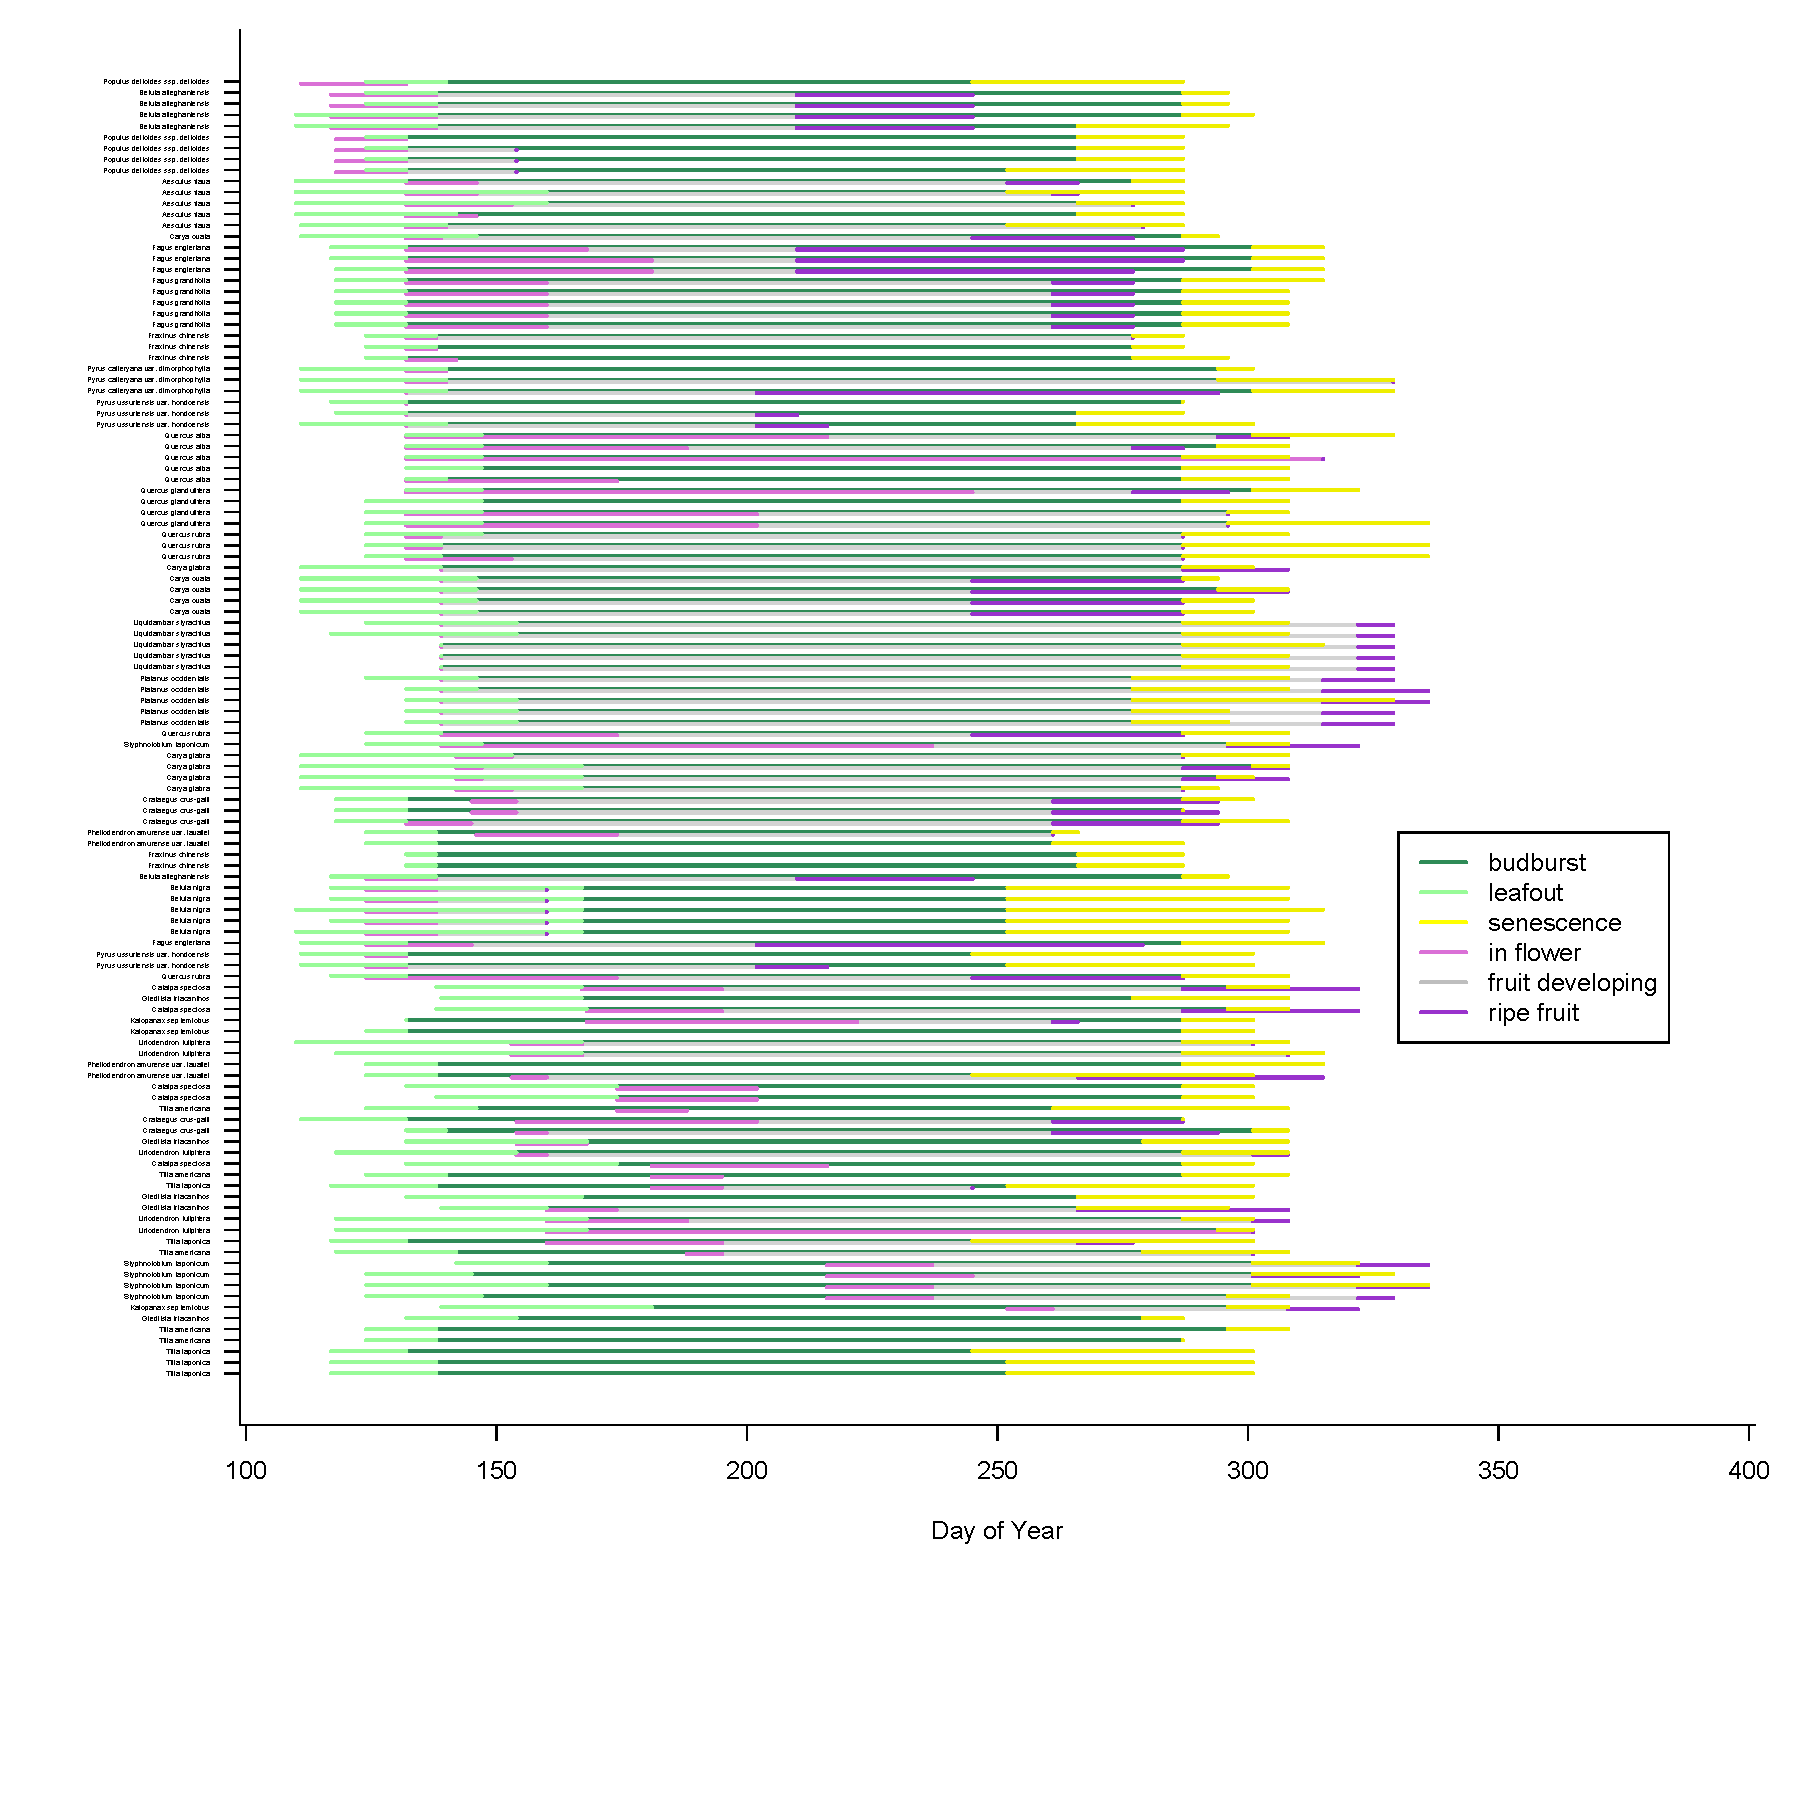
\includegraphics{../analyses/figures/grosea_repsort_ripefruit_ind_legend.pdf}
  \caption{\textbf{Individual tree phenology during the 2015 growing season, ordered by species-level mean first-flower dates.} Growth phenology is shown for budburst (from its mean start day-of-year to the mean start day-of-year for leafout, across all individuals within a species), leafout (from the mean day-of-year when fully-expanded leaves were first observed through the start of senescence), and senescence (from the mean day-of-year when leaves first began changing color through the mean day-of-year when more than 95\% of leaves on the tree had changed color). Reproductive phenology is shown for flowering (from the mean day-of-year when flowers first appeared to the mean day-of-year when fruits first appeared, across all individuals within a species) and fruiting (from the mean day-of-year when fruits first appeared to the mean day-of-year when more than 95\% of fruits were first observed as ripe).}
 \label{fig:focind}
\end{figure}
  
%%%%%%%%%%%%%%%%%%%%%%%%%%%%%%%%%%%%%%%%
\end{document}
%%%%%%%%%%%%%%%%%%%%%%%%%%%%%%%%%%%%%%%%
